\chapter{Des particules à un champ quantique simple}

Reprenons la construction du champ quantique simple, mais sous un angle un peu différent. Deux voies mènent à la théorie quantique des champs. On peut partir des particules et découvrir pourquoi le champ en est le langage naturel, ou partir d’un champ ondulatoire et découvrir pourquoi ses excitations se présentent sous forme de quanta. Ces deux voies sont utiles. Nous suivrons ici la première.

La mécanique quantique ordinaire peut décrire une particule, deux particules ou tout autre nombre fixé de particules. La nature ne respecte pas cette restriction. Le nombre de photons dans une pièce change chaque fois que les lampes émettent ou absorbent du rayonnement. Les particules instables se désintègrent. Dans la désintégration bêta, par exemple,
\begin{equation}
n\longrightarrow p+e^-+\bar{\nu}_e,
\end{equation}
les populations de plusieurs espèces de particules changent donc simultanément. Nous voulons par conséquent une mécanique quantique assez vaste pour englober tout nombre d’occupation possible et, à terme, les processus qui font passer d’un tel nombre à un autre.

Pour l’instant, simplifions fortement le problème. Il n’y a qu’une seule espèce de particule non relativiste. Nous allons d’abord élargir son espace d’états pour qu’il puisse accueillir un nombre quelconque de particules, puis nous aborderons d’autres espèces, la relativité, la diffusion et la désintégration. Les mathématiques ne sont pas particulièrement difficiles, mais le changement de point de vue est abstrait. Mieux vaut avancer assez lentement pour que les notations ne masquent pas l’idée.

\section{Le point de départ : une particule}

Partons d’une particule dans un état \(|\psi\rangle\). Sa fonction d’onde dans l’espace des positions est
\begin{equation}
\psi(x)=\langle x|\psi\rangle.
\label{eq:l07-wavefunction}
\end{equation}
Cette fonction \(\psi\) en minuscule est une fonction ordinaire à valeurs complexes. Ce n’est pas encore un champ quantique ni un opérateur agissant sur un espace d’états à plusieurs particules.

La règle de Born affirme que
\begin{equation}
\rho_\psi(x)=|\psi(x)|^2=\psi^*(x)\psi(x)
\label{eq:l07-born-density}
\end{equation}
est la densité de probabilité de trouver la particule en \(x\). Pour un état normalisé,
\begin{equation}
\int dx\,\psi^*(x)\psi(x)=1.
\label{eq:l07-one-particle-normalization}
\end{equation}
Le membre de droite est la probabilité totale. Comme ce problème contient exactement une particule, cette probabilité est aussi égale au nombre de particules. Cette coïncidence, triviale ici, constituera un indice utile par la suite.

\begin{classroomqa}
\lecturetimestamp{00:09:13}
\audiencequestion{Pourquoi la densité de probabilité doit-elle avoir la forme \(\psi^*(x)\psi(x)\) ?}
\lecturerresponse{C’est la règle de Born, l’un des postulats de la mécanique quantique. L’amplitude associée au résultat de position \(x\) est \(\langle x|\psi\rangle\) ; la densité de probabilité est son carré du module. Cette règle ne se déduit pas de la construction du champ présentée plus loin.}
\end{classroomqa}

\section{Modes, orthogonalité et complétude}

Il existe de nombreuses bases utiles de l’espace de Hilbert à une particule. Les états propres de position constituent une base. Les états propres de tout opérateur hermitien en constituent une autre, sous réserve des précautions habituelles liées aux dégénérescences et aux spectres continus. Comme l’énergie va bientôt jouer un rôle, choisissons un ensemble complet orthonormé d’états propres d’énergie à une particule :
\begin{equation}
|1\rangle,\ |2\rangle,\ldots,
\qquad
\psi_i(x)=\langle x|i\rangle.
\end{equation}

La particule dans une boîte rend l’indice \(i\) concret. La fonction d’onde de l’état fondamental ne possède aucun nœud intérieur, celle de l’état suivant en possède un, et les états d’énergie plus élevée oscillent plus rapidement. Dans un puits carré infini idéal, ce sont essentiellement des ondes sinusoïdales.

\begin{figure}[htbp]
\centering
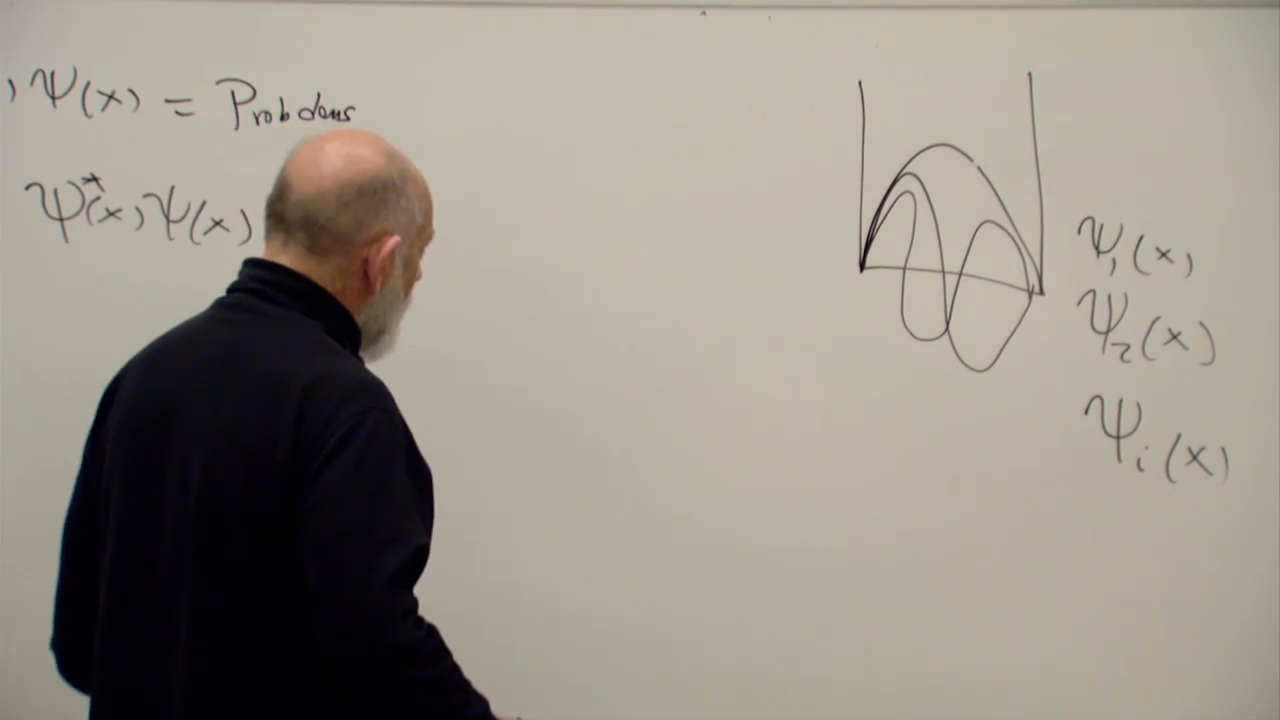
\includegraphics[width=0.94\linewidth]{lecture_07_frame_01.png}
\caption{Les modes de la boîte au tableau pendant le cours. À gauche, on distingue encore la densité de Born et la normalisation à une particule ; à droite, le puits montre \(\psi_1(x)\), \(\psi_2(x)\) et l’étiquette générale \(\psi_i(x)\).}
\lectureframe{00:08:25}
\end{figure}

On peut dégager la même structure modale de ce qui masque le tableau pendant le cours :
\begin{figure}[htbp]
\centering
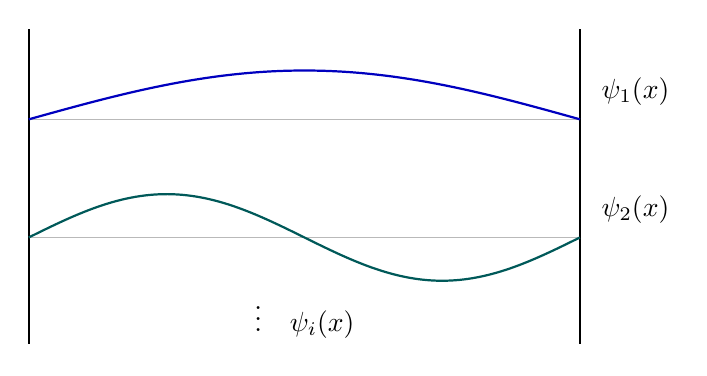
\begin{tikzpicture}[x=1cm,y=1cm]
  \draw[thick] (0,0) -- (0,4.0);
  \draw[thick] (7,0) -- (7,4.0);
  \draw[gray!55] (0,2.85) -- (7,2.85);
  \draw[gray!55] (0,1.35) -- (7,1.35);
  \draw[blue!75!black,thick,domain=0:7,samples=120]
    plot (\x,{2.85+0.62*sin(180*\x/7)});
  \draw[teal!70!black,thick,domain=0:7,samples=120]
    plot (\x,{1.35+0.55*sin(360*\x/7)});
  \node[right] at (7.15,3.20) {$\psi_1(x)$};
  \node[right] at (7.15,1.70) {$\psi_2(x)$};
  \node at (3.5,0.38) {$\vdots\quad\psi_i(x)$};
\end{tikzpicture}
\caption{Reconstitution épurée du schéma qualitatif de la boîte. Les décalages verticaux servent uniquement à séparer les deux fonctions d’onde pour les représenter.}
\end{figure}

L’orthonormalité s’écrit
\begin{equation}
\int dx\,\psi_i^*(x)\psi_j(x)=\delta_{ij}.
\label{eq:l07-orthonormality}
\end{equation}
Si \(i=j\), l’état est normalisé et l’intégrale vaut un. Si \(i\ne j\), les deux états sont orthogonaux et l’intégrale s’annule.

La complétude est une affirmation tout aussi importante :
\begin{equation}
\sum_i |i\rangle\langle i|=\mathbf 1.
\label{eq:l07-resolution}
\end{equation}
Chaque \(|i\rangle\langle i|\) projette sur une direction de la base ; la somme sur la base complète est l’identité. Appliquée à un vecteur quelconque, elle décompose simplement ce vecteur en ses composantes, puis le reconstitue.

Insérons maintenant l’équation~\eqref{eq:l07-resolution} entre deux états de position :
\begin{align}
\langle y|x\rangle
&=\sum_i\langle y|i\rangle\langle i|x\rangle \\
&=\sum_i\psi_i(y)\psi_i^*(x) \\
&=\delta(y-x).
\label{eq:l07-position-completeness}
\end{align}
L’astérisque porte sur le facteur dont l’ordre dans le bra-ket est \(\langle i|x\rangle\). Inverser \(x\) et \(y\) donne une forme équivalente, complexe conjuguée. Ainsi, toute base complète orthonormée fournit une représentation de la fonction delta. Les sinus, les cosinus, les fonctions d’onde de l’oscillateur et les fonctions propres d’énergie remplissent tous ce rôle.

\begin{classroomqa}
\lecturetimestamp{00:13:43}
\audiencequestion{La deuxième fonction d’onde de la somme de complétude doit-elle porter le complexe conjugué ?}
\lecturerresponse{Oui. Dans l’ordre \(\langle y|i\rangle\langle i|x\rangle\), les facteurs sont \(\psi_i(y)\psi_i^*(x)\). Garder visible l’ordre du bra-ket évite de deviner ou de mal placer l’astérisque.}
\end{classroomqa}

Voilà les mathématiques à une particule dont nous aurons besoin. Changeons maintenant d’espace d’états.

\section{L’espace de Fock comme espace d’états élargi}

Pour plusieurs particules identiques, une base commode indique combien de particules occupent chaque mode à une particule :
\begin{equation}
|n_1,n_2,n_3,\ldots\rangle.
\label{eq:l07-fock-basis}
\end{equation}
L’entier \(n_i\) est le nombre d’occupation du mode \(i\). Ce ket n’est pas un état à une particule écrit dans une notation plus sophistiquée. Il appartient à un espace de Hilbert plus vaste qui contient le secteur à zéro particule, tous les états à une particule, tous les états à deux particules, et ainsi de suite. Cet espace élargi s’appelle l’espace de Fock.

Pour modifier les occupations, introduisons, pour chaque mode, un opérateur de création et un opérateur d’annihilation :
\begin{equation}
a_i^\dagger,\qquad a_i.
\end{equation}
Le premier ajoute une particule au mode \(i\), tandis que le second en enlève une. À ce stade, le langage de l’oscillateur harmonique sert d’outil de comptabilité : il n’est pas nécessaire qu’un ressort oscille littéralement. L’algèbre de l’oscillateur fournit exactement les outils nécessaires pour augmenter ou diminuer les nombres d’occupation.

L’opérateur nombre du mode est
\begin{equation}
\begin{aligned}
N_i&=a_i^\dagger a_i,\\
N_i|n_1,\ldots,n_i,\ldots\rangle
&=n_i|n_1,\ldots,n_i,\ldots\rangle.
\end{aligned}
\end{equation}
Le vide est
\begin{equation}
|0\rangle\equiv|0,0,0,\ldots\rangle,
\qquad
a_i|0\rangle=0
\quad\text{for every }i.
\label{eq:l07-vacuum}
\end{equation}
Un état à une particule dans le mode \(i\) est donc
\begin{equation}
|i\rangle=a_i^\dagger|0\rangle.
\label{eq:l07-mode-created}
\end{equation}
Le même symbole \(|i\rangle\) peut désormais désigner soit un vecteur de base à une particule, soit ce vecteur intégré au secteur à une particule de l’espace de Fock. Cette intégration est donnée par l’équation~\eqref{eq:l07-mode-created} ; le contexte indique l’espace considéré.

\section{Réunir les modes dans un champ}

Définissons les champs d’annihilation et de création par
\begin{equation}
\Psi(x)=\sum_i \psi_i(x)a_i,
\qquad
\Psi^\dagger(x)=\sum_i \psi_i^*(x)a_i^\dagger.
\label{eq:l07-field-expansion}
\end{equation}
La majuscule est importante. Les fonctions \(\psi_i(x)\) minuscules sont des nombres complexes ; la majuscule \(\Psi(x)\) désigne un opérateur sur l’espace de Fock. En chaque point de l’espace \(x\), l’équation~\eqref{eq:l07-field-expansion} donne une combinaison linéaire différente des opérateurs de mode. C’est cela qu’on entend par fonction opératorielle de la position.

Pour des particules libres, les fonctions de mode peuvent être des ondes planes \(e^{ikx}\). L’équation~\eqref{eq:l07-field-expansion} est alors un développement de Fourier, à ceci près que ses coefficients de Fourier sont des opérateurs plutôt que des nombres. L’ancienne terminologie appelle les nombres complexes ordinaires des nombres \(c\) et les opérateurs quantiques des nombres \(q\). Les fonctions de mode sont des nombres \(c\) et commutent avec tout ; les opérateurs \(a_i\) et \(a_i^\dagger\) portent le caractère opératoriel.

Ni \(\Psi\) ni \(\Psi^\dagger\) n’est hermitien. Ils sont adjoints l’un de l’autre. Les deux combinaisons
\begin{equation}
\Psi+\Psi^\dagger,
\qquad
i(\Psi^\dagger-\Psi)
\label{eq:l07-hermitian-combinations}
\end{equation}
sont hermitiennes et peuvent représenter des observables. Pour l’instant, toutefois, les champs sont surtout utiles comme outils pour créer, annihiler et compter des particules localement.

\begin{classroomqa}
\lecturetimestamp{00:21:05}
\audiencequestion{Que signifie le fait qu’un opérateur dépende de \(x\) ?}
\lecturerresponse{Cela signifie que chaque valeur de \(x\) sélectionne un opérateur différent. La dépendance spatiale est portée par les fonctions de mode ordinaires, tandis que chaque combinaison linéaire obtenue agit sur le même espace de Fock.}
\end{classroomqa}

\section{Ce que fait le champ de création}

Une définition devient utile lorsqu’on demande ce qu’elle fait. Partons d’un état propre de position dans le secteur à une particule et insérons la résolution de l’identité :
\begin{align}
|x\rangle
&=\sum_i |i\rangle\langle i|x\rangle \\
&=\sum_i a_i^\dagger|0\rangle\,\psi_i^*(x) \\
&=\Psi^\dagger(x)|0\rangle.
\label{eq:l07-local-creation}
\end{align}
Ainsi, \(a_i^\dagger\) crée une particule dans le mode bien défini \(i\), tandis que \(\Psi^\dagger(x)\) crée une particule localisée en \(x\). Dans la base de position idéalisée, cette localisation est au sens des distributions ; une préparation physique utiliserait un paquet d’ondes étroit, mais le sens algébrique est le même.

\begin{classroomqa}
\lecturetimestamp{00:24:48}
\audiencequestion{\(\sum_i|i\rangle\langle i|\) est-il un projecteur ?}
\lecturerresponse{Chaque terme est un projecteur sur un état de base. La somme complète est l’identité elle-même et s’appelle une résolution de l’identité. Son insertion ne modifie pas l’état, mais rend visibles ses composantes dans la base choisie.}
\end{classroomqa}

L’équation~\eqref{eq:l07-local-creation} donne la première interprétation directe du champ en termes de particules. Nous n’avons pas simplement accolé une étiquette spatiale à un opérateur abstrait. Nous avons construit l’opération qui crée une particule en ce point de l’espace.

\begin{classroomqa}
\lecturetimestamp{00:28:20}
\audiencequestion{Le champ de création dans l’espace des positions doit-il porter un astérisque ou une dague ?}
\lecturerresponse{Pour l’adjoint d’un opérateur, utilisez une dague. Les astérisques désignent le complexe conjugué des fonctions d’onde ordinaires \(\psi_i(x)\) ; les dagues se placent sur \(a_i^\dagger\) et \(\Psi^\dagger(x)\).}
\end{classroomqa}

\begin{classroomqa}
\lecturetimestamp{00:28:36}
\audiencequestion{Peut-on déplacer les opérateurs de création de part et d’autre des fonctions d’onde dans le développement en modes ?}
\lecturerresponse{Oui. Les \(\psi_i(x)\) sont des nombres \(c\) et commutent donc avec tout opérateur. Il faut seulement faire attention lorsqu’on change l’ordre d’opérateurs qui ne commutent pas, tels que \(a_i\) et \(a_j^\dagger\).}
\end{classroomqa}

\section{De la densité de probabilité à la densité de particules}

Jouons maintenant avec le champ. L’expression qui vient naturellement est
\begin{equation}
\int dx\,\Psi^\dagger(x)\Psi(x).
\end{equation}
Elle ressemble à l’intégrale de normalisation à une particule, mais ses facteurs sont désormais des opérateurs. Insérons les développements en modes sans en modifier l’ordre :
\begin{align}
\int dx\,\Psi^\dagger(x)\Psi(x)
&=\int dx
\left(\sum_i a_i^\dagger\psi_i^*(x)\right)\\
&\qquad\times\left(\sum_j a_j\psi_j(x)\right) \\
&=\sum_{i,j}a_i^\dagger a_j
\int dx\,\psi_i^*(x)\psi_j(x) \\
&=\sum_{i,j}a_i^\dagger a_j\,\delta_{ij} \\
&=\sum_i a_i^\dagger a_i.
\label{eq:l07-number-derivation}
\end{align}
L’opérateur nombre total est donc
\begin{equation}
N=\sum_i N_i
=\int dx\,\Psi^\dagger(x)\Psi(x).
\label{eq:l07-total-number}
\end{equation}
Pour les états considérés, les occupations des excitations d’énergie finie décroissent à haute énergie de mode, si bien que ce total est en général fini, même si l’ensemble des modes possibles est infini.

L’intégrande est l’opérateur de densité locale de particules :
\begin{equation}
n(x)=\Psi^\dagger(x)\Psi(x).
\label{eq:l07-density}
\end{equation}
À proprement parler, on ne mesure pas la densité en un point mathématique. Pour une petite région \(R\), on mesure
\begin{equation}
N_R=\int_R dx\,n(x),
\label{eq:l07-regional-number}
\end{equation}
le nombre de particules dans cette région. Comme toute observable quantique, \(N_R\) n’a pas nécessairement de valeur déterminée dans un état arbitraire. Des préparations répétées peuvent donner des résultats différents.

\begin{classroomqa}
\lecturetimestamp{00:36:27}
\audiencequestion{\(\Psi^\dagger(x)\Psi(x)\) est-elle la densité de probabilité à plusieurs particules ?}
\lecturerresponse{Son interprétation directe est celle d’une densité de particules. Une amplitude de probabilité à plusieurs particules dépend généralement de toutes les coordonnées des particules. La forme bilinéaire locale, elle, compte les particules dans une petite région lorsqu’on l’intègre sur cette région.}
\end{classroomqa}

\begin{classroomqa}
\lecturetimestamp{00:38:28}
\audiencequestion{Les opérateurs \(a_i\) et \(a_i^\dagger\) agissent-ils uniquement sur les vecteurs d’état, et pas sur les fonctions d’onde à une particule ?}
\lecturerresponse{Oui. Ils agissent sur les états de l’espace de Fock, tels que \(|n_1,n_2,\ldots\rangle\). Les fonctions de mode à une particule qui les multiplient sont des nombres ordinaires, et ces opérateurs d’échelle n’agissent pas sur elles.}
\end{classroomqa}

Les kets d’occupation forment une base, mais ne constituent pas l’état le plus général. On peut les superposer, y compris de façon à répartir différemment un même nombre total de particules entre les modes. Pour des espèces neutres comme les photons, on peut aussi superposer des secteurs ayant des nombres totaux de particules différents. L’opérateur de l’équation~\eqref{eq:l07-regional-number} conserve la même signification opérationnelle dans chacun de ces états.

\begin{classroomqa}
\lecturetimestamp{00:40:01}
\audiencequestion{Si l’on divise la densité de particules par le nombre total, obtient-on la densité de probabilité de trouver une particule en \(x\) ?}
\lecturerresponse{Dans une situation à \(N\) fixé et à grand nombre de particules, \(N_R/N\) est une fréquence relative et suit généralement de très près une probabilité à une particule. Il ne s’agit pas d’une identité opératorielle qui ferait d’un résultat de mesure une probabilité. Le nombre mesuré fluctue, typiquement d’une quantité de l’ordre de \(\sqrt N\) dans un modèle de particules indépendantes, et un résultat exceptionnel peut s’écarter fortement de la probabilité, même s’il est peu probable.}
\end{classroomqa}

\begin{classroomqa}
\lecturetimestamp{00:42:25}
\audiencequestion{Qu’advient-il de la conservation de la charge dans une superposition d’un état à un électron et d’un état sans électron ?}
\lecturerresponse{Ce n’est pas le type de superposition utilisé dans un secteur fermé de charge électrique fixée. On peut superposer différentes répartitions qui ont la même charge totale. Les photons n’ayant pas de charge électrique, les secteurs de nombre de photons différents ne posent pas ce problème. Le nombre d’électrons et de positrons peut aussi varier simultanément tout en conservant la charge nette.}
\end{classroomqa}

\section{Énergie de particules indépendantes}

L’énergie est la prochaine observable. Commençons par nous limiter à des particules qui n’interagissent pas entre elles. Cette approximation est souvent bonne dans un système dilué. Même les photons interagissent en principe par des processus d’ordre supérieur, mais le rayonnement ordinaire en laboratoire est assez dilué pour que la description par des particules indépendantes soit excellente.

Notons \(\omega_i\) l’énergie d’une particule dans le mode \(i\), avec \(\hbar=1\). Un mode désigne un état à une particule. L’hamiltonien total est alors
\begin{equation}
H=\sum_i\omega_i N_i
=\sum_i\omega_i a_i^\dagger a_i.
\label{eq:l07-mode-hamiltonian}
\end{equation}
Chaque mode occupé contribue son énergie à une particule une fois par particule.

\begin{classroomqa}
\lecturetimestamp{00:48:16}
\audiencequestion{\(\omega_i\) est-elle une fonction de la position ?}
\lecturerresponse{Non. C’est la valeur propre d’énergie associée au mode \(i\). La fonction \(\psi_i(x)\) dépend de la position ; \(\omega_i\) dépend du niveau d’énergie sélectionné.}
\end{classroomqa}

Les valeurs \(\omega_i\) sont déterminées par l’équation de Schrödinger indépendante du temps à une particule. Définissons
\begin{equation}
h=-\frac{\nabla^2}{2m}+V(x).
\label{eq:l07-one-particle-h}
\end{equation}
On a alors
\begin{equation}
h\psi_i(x)=\omega_i\psi_i(x).
\label{eq:l07-schrodinger-eigenvalue}
\end{equation}
En une dimension, l’opérateur quantité de mouvement est \(p=-i\partial_x\), et \(p^2/(2m)\) devient \(-\partial_x^2/(2m)\). En trois dimensions, les trois dérivées secondes se combinent en \(-\nabla^2/(2m)\).

\begin{figure}[htbp]
\centering
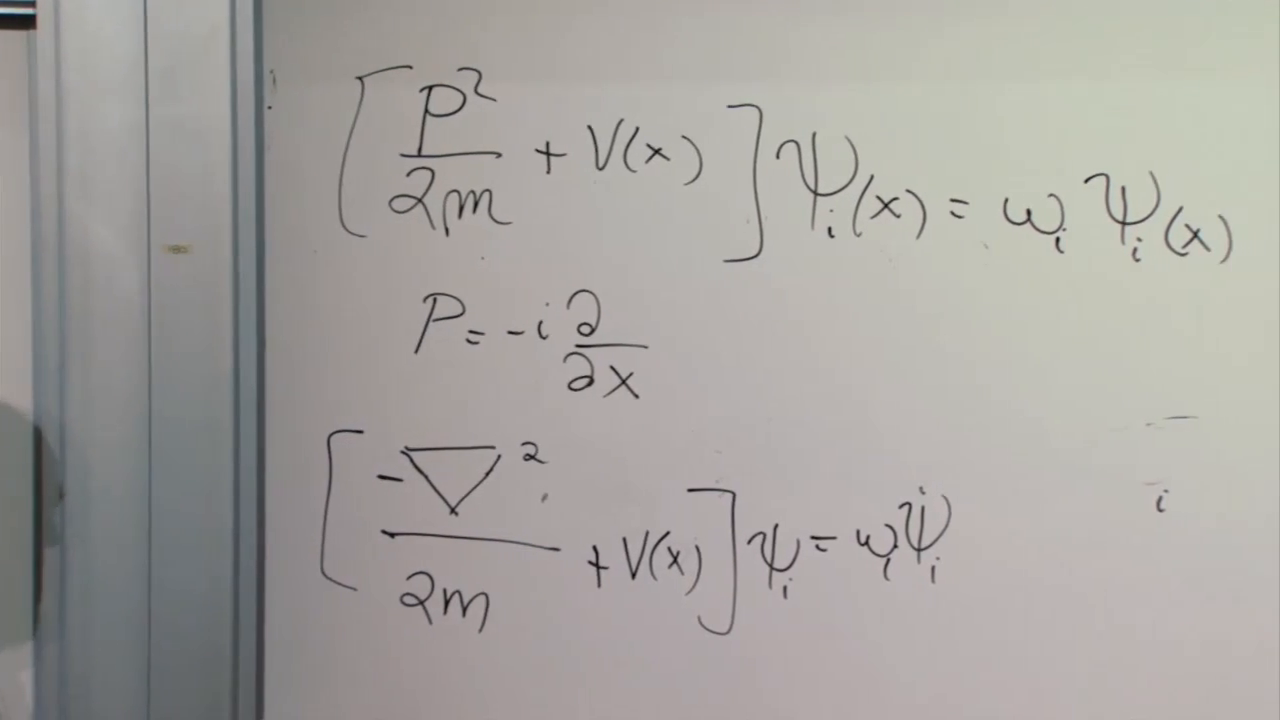
\includegraphics[width=0.94\linewidth]{lecture_07_frame_02.png}
\caption{Passage au tableau de \(p^2/(2m)+V(x)\) à la forme différentielle de l’équation aux valeurs propres de Schrödinger à une particule. L’équation~\eqref{eq:l07-schrodinger-eigenvalue} en est une reconstitution épurée.}
\lectureframe{00:54:10}
\end{figure}

Pour une fonction d’onde à une particule normalisée quelconque, la valeur moyenne usuelle est
\begin{equation}
\langle h\rangle_\psi
=\int dx\,\psi^*(x)h\psi(x).
\label{eq:l07-one-particle-energy-expectation}
\end{equation}
On peut conjecturer la formule à plusieurs particules en remplaçant la fonction d’onde minuscule par le champ à valeurs opératorielles. Ce n’est pas encore une démonstration, mais la conjecture dont nous allons vérifier la validité :
\begin{equation}
H=\int dx\,\Psi^\dagger(x)h\Psi(x).
\label{eq:l07-field-hamiltonian}
\end{equation}

\section{Écrire d’abord le résultat, puis le démontrer}

Insérons l’équation~\eqref{eq:l07-field-expansion} dans l’hamiltonien proposé :
\begin{align}
\int dx\,\Psi^\dagger h\Psi
&=\int dx
\left(\sum_i a_i^\dagger\psi_i^*(x)\right)
h\left(\sum_j a_j\psi_j(x)\right) \\
&=\sum_{i,j}a_i^\dagger a_j
\int dx\,\psi_i^*(x)h\psi_j(x).
\label{eq:l07-h-expanded}
\end{align}
L’opérateur différentiel \(h\) agit sur la fonction d’onde \(\psi_j(x)\) qui dépend de \(x\), et non sur l’opérateur de mode \(a_j\). D’après l’équation de Schrödinger,
\begin{equation}
h\psi_j(x)=\omega_j\psi_j(x).
\end{equation}
Il s’ensuit que
\begin{align}
\int dx\,\Psi^\dagger h\Psi
&=\sum_{i,j}a_i^\dagger a_j\omega_j
\int dx\,\psi_i^*(x)\psi_j(x) \\
&=\sum_{i,j}a_i^\dagger a_j\omega_j\delta_{ij} \\
&=\sum_j\omega_j a_j^\dagger a_j.
\label{eq:l07-h-proof}
\end{align}
C’est précisément l’équation~\eqref{eq:l07-mode-hamiltonian}. L’expression locale du champ et la somme des énergies de toutes les particules désignent le même opérateur.

\begin{figure}[htbp]
\centering
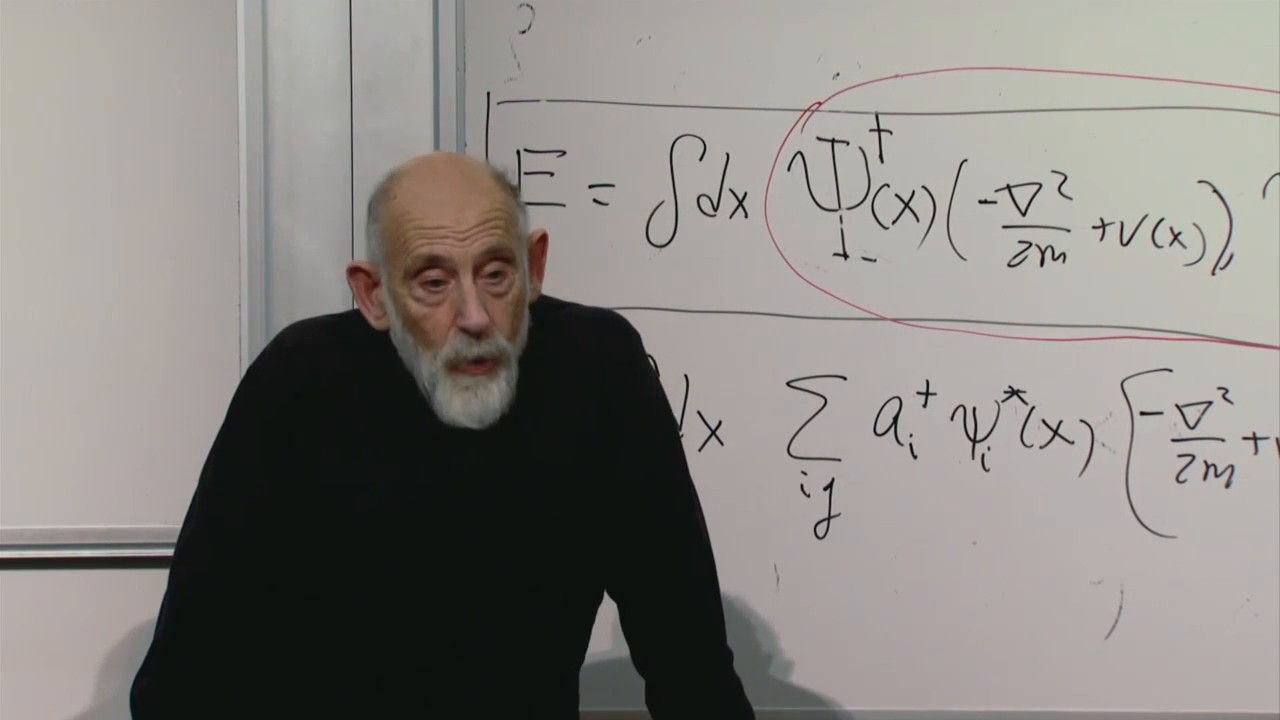
\includegraphics[width=0.94\linewidth]{lecture_07_frame_03.png}
\caption{L’hamiltonien du champ mis en évidence au tableau, avec le début de la démonstration par développement en modes en dessous. L’image prise pendant le cours est conservée comme élément de preuve ; les équations~\eqref{eq:l07-field-hamiltonian}--\eqref{eq:l07-h-proof} rétablissent tout le calcul.}
\lectureframe{01:05:34}
\end{figure}

Dans cette démonstration, aucun opérateur de création n’a été commuté avec un opérateur d’annihilation. L’ordre \(a_i^\dagger a_j\) est conservé du début à la fin. Seules les fonctions d’onde, nombres \(c\), et leurs valeurs propres sont déplacées librement.

\section{Pourquoi s’agit-il d’un champ ?}

Pourquoi appeler \(\Psi(x)\) un champ ? Parce qu’il s’agit d’une grandeur à valeurs opératorielles définie en chaque point de l’espace, et que les combinaisons hermitiennes ou les formes bilinéaires qu’on en construit sont des observables locales. La densité \(n(x)\) et l’expression locale de l’énergie présentée plus loin en sont deux exemples. Le mot ne cache aucun autre critère mathématique.

Ce champ n’est pas le champ électromagnétique. Il décrit l’espèce non relativiste dont proviennent les modes et l’hamiltonien à une particule \(p^2/(2m)+V\) : par exemple des atomes lents, des neutrons, des protons ou des électrons. Ces particules sont les quanta de leur champ respectif, au même sens structurel que les photons sont les quanta du champ électromagnétique.

\begin{classroomqa}
\lecturetimestamp{01:02:45}
\audiencequestion{À quel moment un champ intervient-il dans le passage du système à plusieurs particules à la formule ci-dessus ?}
\lecturerresponse{Il intervient dans l’équation~\eqref{eq:l07-field-expansion} : \(\Psi(x)\) est un opérateur en chaque point de l’espace. Les dérivations qui suivent montrent que ses produits locaux mesurent les densités de particules et d’énergie. Dépendance en position et contenu opératoriel : voilà précisément la structure de champ que nous construisons.}
\end{classroomqa}

\section{Densité locale d’énergie}

L’équation~\eqref{eq:l07-field-hamiltonian} exprime l’énergie totale comme une intégrale sur l’espace :
\begin{equation}
\begin{aligned}
H&=\int dx\,\mathcal H(x),\\
\mathcal H(x)
&=-\frac{1}{2m}\Psi^\dagger(x)\nabla^2\Psi(x)\\
&\quad+V(x)\Psi^\dagger(x)\Psi(x).
\end{aligned}
\label{eq:l07-hamiltonian-density}
\end{equation}
L’intégrande constitue une densité locale d’énergie naturelle pour cet hamiltonien. Sa forme locale n’est pas unique. Par exemple, une intégration par parties remplace le terme cinétique par
\begin{equation}
\mathcal H_{\rm kin}(x)
=\frac{1}{2m}\nabla\Psi^\dagger(x)\mathbin{\cdot}\nabla\Psi(x)
\label{eq:l07-kinetic-density}
\end{equation}
à un terme de bord près. Les deux expressions donnent le même hamiltonien total sous les conditions aux limites habituelles. C’est la petite ambiguïté mentionnée dans le cours.

\begin{classroomqa}
\lecturetimestamp{01:05:57}
\audiencequestion{Faut-il intégrer la densité d’énergie sur tout l’espace ?}
\lecturerresponse{L’intégration sur tout l’espace donne l’énergie totale. L’intégration sur une région plus petite donne l’énergie attribuée à cette région, sous réserve de l’ambiguïté habituelle dans le choix d’une densité locale dont l’intégrale sur tout l’espace donne le même hamiltonien.}
\end{classroomqa}

\begin{classroomqa}
\lecturetimestamp{01:06:25}
\audiencequestion{En quoi la majuscule \(N_i\) de la formule de l’énergie diffère-t-elle de la minuscule \(n_i\) ?}
\lecturerresponse{\(N_i=a_i^\dagger a_i\) est un opérateur. L’entier \(n_i\) est l’une de ses valeurs propres sur un état de nombre d’occupation. Les opérateurs agissent sur des états ; leurs valeurs propres sont des nombres ordinaires.}
\end{classroomqa}

\begin{classroomqa}
\lecturetimestamp{01:06:46}
\audiencequestion{Peut-on écrire l’hamiltonien du champ lui-même sous forme de bra ou de ket dans la notation de Dirac ?}
\lecturerresponse{Non. Les bras et les kets désignent des vecteurs d’état et leurs éléments duaux. Le champ et l’hamiltonien sont des opérateurs agissant sur ces états. Une valeur moyenne telle que \(\langle\Phi|H|\Phi\rangle\) fait intervenir les deux types d’objets, qu’il ne faut pas confondre.}
\end{classroomqa}

\section{Retrouver une particule et approcher un champ classique}

Le formalisme élargi contient la mécanique quantique ordinaire à une particule. Restreignons l’espace de Fock aux états qui satisfont à
\begin{equation}
N|\Phi\rangle=|\Phi\rangle.
\end{equation}
Dans ce secteur, la construction du champ reproduit tous les états à une particule et toutes les prédictions à une particule. Nous n’avons pas remplacé l’ancienne théorie ; nous l’avons intégrée dans un espace qui permet aussi de décrire zéro, deux ou un nombre quelconque de particules.

À l’autre extrême, un mode occupé par un très grand nombre de bosons peut se comporter approximativement comme une onde classique. Dans des états cohérents ou semi-classiques appropriés, la valeur moyenne
\begin{equation}
\Phi_{\rm cl}(x,t)=\langle\Psi(x,t)\rangle
\end{equation}
satisfait l’équation d’allure classique
\begin{equation}
i\partial_t\Phi_{\rm cl}(x,t)
=\left(-\frac{\nabla^2}{2m}+V(x)\right)\Phi_{\rm cl}(x,t)
\label{eq:l07-classical-schrodinger}
\end{equation}
pour la théorie libre non relativiste. Le cours énonce ce lien sans le démontrer. Il fait le pont entre un ensemble de quanta et un champ ondulatoire : les grandes occupations réduisent les fluctuations relatives et font que certaines valeurs moyennes se comportent classiquement.

Le formalisme relève donc à la fois de la comptabilité et de la physique. Il organise tous les secteurs de nombre de particules, tout en décrivant l’interférence, l’intrication et l’émergence d’ondes classiques à partir de particules quantiques.

\begin{classroomqa}
\lecturetimestamp{01:10:43}
\audiencequestion{Pourquoi peut-on manipuler les opérateurs de création et d’annihilation dans l’intégrale presque comme des nombres ordinaires ?}
\lecturerresponse{On ne les a jamais permutés l’un avec l’autre. Les fonctions de mode ordinaires commutent avec eux, et les dérivées agissent uniquement sur ces fonctions. Faire passer un opérateur d’annihilation à travers un opérateur de création nécessiterait d’utiliser le commutateur et pourrait ajouter un terme ; aucune étape de la démonstration n’effectue cette permutation.}
\end{classroomqa}

\section{Parenthèse sur la notation de Dirac}

Une partie de la confusion est historique. Une fonction d’onde à une particule satisfait une équation d’onde et ressemble superficiellement à un champ classique, tout en étant une amplitude de probabilité. Les débuts de la théorie quantique ont dû dissocier ces rôles, puis expliquer comment les champs ondulatoires réellement mesurables, comme l’électromagnétisme, sont constitués de quanta. L’espace de Fock et les champs à valeurs opératorielles résolvent ce conflit apparent.

La notation de Dirac rend cette distinction particulièrement concise. Un ket appartient à un espace vectoriel, un bra à son dual, et leur juxtaposition forme un produit scalaire. La résolution
\begin{equation}
\sum_i|i\rangle\langle i|=\mathbf 1
\end{equation}
devient alors presque limpide. Le cours l’illustre par une anecdote tirée d’un enseignement de mécanique quantique à des mathématiciens : le contenu mathématique leur était déjà familier, mais la notation rendait les manipulations usuelles si transparentes que la structure semblait nouvelle. L’idée n’est pas qu’une discipline ignorait le concept. C’est qu’une notation bien choisie rend difficile la confusion entre les opérations autorisées.

Cette leçon est importante ici. Il existe maintenant plusieurs opérateurs distincts :
\begin{itemize}
\item \(h\) agit sur les fonctions d’onde à une particule comme un opérateur différentiel ;
\item \(a_i\) et \(a_i^\dagger\) agissent sur les états de nombre d’occupation dans l’espace de Fock ;
\item \(\Psi(x)\), \(\Psi^\dagger(x)\), \(N\) et \(H\) agissent eux aussi sur l’espace de Fock.
\end{itemize}
Le développement de l’équation~\eqref{eq:l07-field-expansion} relie les deux premiers cadres sans les confondre.

\begin{classroomqa}
\lecturetimestamp{01:18:16}
\audiencequestion{Les champs ne sont-ils qu’un formalisme pour décrire des ensembles de particules ?}
\lecturerresponse{C’est un formalisme, mais il n’est pas vide de contenu. Ses observables locales sont mesurables, et les particules sont des objets quantiques qui présentent interférence et intrication, et non des boulettes classiques. Les opérateurs de champ encodent précisément ces propriétés collectives mesurables.}
\end{classroomqa}

\section{Prudence relativiste et aparté sur l’électromagnétisme}

La construction présentée jusqu’ici est non relativiste. En physique relativiste, la quantité de mouvement reste un bon label des particules, mais la localisation précise de leur position est beaucoup plus délicate. Par conséquent, une densité locale de nombre de photons n’est généralement pas une notion aussi nette que \(n(x)\) dans le cas non relativiste. La densité d’énergie reste bien définie et constitue l’observable locale la plus sûre.

Le cours propose une analogie électromagnétique utile, explicitement heuristique. Regroupons les champs électrique et magnétique dans le vecteur complexe
\begin{equation}
\mathbf F=\mathbf E+i\mathbf B,
\qquad
\mathbf F^*=\mathbf E-i\mathbf B.
\label{eq:l07-riemann-silberstein}
\end{equation}
On a alors
\begin{equation}
\mathbf F^*\mathbin{\cdot}\mathbf F
=\mathbf E^2+\mathbf B^2,
\label{eq:l07-em-density}
\end{equation}
qui est proportionnel à la densité d’énergie électromagnétique dans les unités conventionnelles. Il ne s’agit pas littéralement d’une densité de probabilité des photons. Il vaut mieux y voir une variable de champ compacte dont le carré du module mesure la densité d’énergie, ou, de manière informelle, une densité de photons pondérée par leur énergie.

\begin{classroomqa}
\lecturetimestamp{01:19:10}
\audiencequestion{Peut-on identifier la densité de photons à l’intensité du champ électrique ?}
\lecturerresponse{Seulement de façon qualitative et avec prudence. Pour des photons relativistes, le nombre local de particules n’est pas la notion à privilégier. L’affirmation robuste est que \(E^2+B^2\) est proportionnel à la densité d’énergie et que la combinaison complexe \(\mathbf E+i\mathbf B\) regroupe les équations de Maxwell sous une forme analogue à celle de Schrödinger.}
\end{classroomqa}

\begin{classroomqa}
\lecturetimestamp{01:20:09}
\audiencequestion{Pourquoi une particule relativiste peut-elle avoir une quantité de mouvement bien définie alors que sa position pose problème ?}
\lecturerresponse{La quantité de mouvement caractérise sans ambiguïté les représentations relativistes à une particule, tandis qu’une localisation stricte entre en conflit avec la création de particules et la description par les champs relativistes. Ce cours ne développe pas cette théorie ; cet avertissement marque la limite de l’interprétation non relativiste de la densité présentée ici.}
\end{classroomqa}

\section{Ordre des opérateurs et constante d’énergie du fondamental}

On ne peut pas modifier l’ordre des opérateurs à la légère. Pour les modes bosoniques,
\begin{equation}
a_i a_i^\dagger=a_i^\dagger a_i+1.
\end{equation}
Par conséquent, remplacer l’ordre normal \(\Psi^\dagger h\Psi\) par l’ordre inversé \((h\Psi)\Psi^\dagger\), ou par la forme correspondante correctement intégrée, ajoute la contribution du commutateur. Dans une base de modes, il s’agit d’une somme additive d’un quantum d’énergie par mode. C’est la constante d’énergie du fondamental, ou énergie du point zéro ; dans un continuum, elle nécessite une régularisation. Le cours n’examine pas cette question ici ; il signale simplement que les deux ordres ne sont pas équivalents.

\begin{classroomqa}
\lecturetimestamp{01:22:04}
\audiencequestion{Que se passe-t-il si \(\Psi\) et \(\Psi^\dagger\) sont intervertis dans l’Hamiltonien ?}
\lecturerresponse{Leur commutateur doit être pris en compte. Inverser leur ordre ajoute donc une contribution à l’état fondamental indépendante de l’état considéré, au lieu de redonner la même expression. L’Hamiltonien affiché est écrit en ordre normal, \(\Psi^\dagger h\Psi\).}
\end{classroomqa}

\section{La quantité de mouvement, dernier test}

Les dernières minutes reprennent une fois de plus la même promotion. Pour une particule,
\begin{equation}
\langle p\rangle_\psi
=\int dx\,\psi^*(x)\left(-i\partial_x\right)\psi(x).
\label{eq:l07-one-particle-momentum}
\end{equation}
En remplaçant la fonction d’onde par le champ, on obtient l’opérateur de quantité de mouvement totale
\begin{equation}
P=\int dx\,\Psi^\dagger(x)\left(-i\partial_x\right)\Psi(x),
\label{eq:l07-field-momentum}
\end{equation}
ou, en trois dimensions,
\begin{equation}
\mathbf P=\int d^3x\,\Psi^\dagger(\mathbf x)
\left(-i\boldsymbol\nabla\right)\Psi(\mathbf x).
\end{equation}
Les champs portent une quantité de mouvement. Un laser suffisamment puissant transfère de la quantité de mouvement à un mur et exerce une force ; dans la description quantique, la quantité de mouvement du champ est la somme des quantités de mouvement des photons.

L’équation~\eqref{eq:l07-field-momentum} est un opérateur, et non une valeur moyenne. À partir d’un état de l’espace de Fock \(|\Phi\rangle\), on peut alors calculer
\begin{equation}
\langle P\rangle_\Phi=\langle\Phi|P|\Phi\rangle.
\end{equation}
Il faut à la fois un opérateur et un état pour former une valeur moyenne. Confondre l’observable avec sa valeur moyenne effacerait précisément la distinction que le cours a établi.

\begin{classroomqa}
\lecturetimestamp{01:26:02}
\audiencequestion{La quantité de mouvement du champ affichée est-elle déjà la quantité de mouvement moyenne ?}
\lecturerresponse{Non. C’est l’opérateur hermitien qui représente l’observable. Il faut fournir un état et placer l’opérateur entre le bra et le ket de cet état pour obtenir une valeur moyenne ; une mesure peut néanmoins fluctuer autour de cette moyenne.}
\end{classroomqa}

C’est le point d’arrêt naturel. À partir des particules, nous avons construit des champs locaux de création et d’annihilation, nous nous en sommes servis pour compter les particules et avons réécrit la somme des énergies et des quantités de mouvement des particules comme des opérateurs de champ. L’étape suivante ne consiste pas à changer encore de notation. Il s’agit de faire représenter des processus physiques par les opérateurs de champ : la désintégration des particules, leur diffusion et les transformations d’une espèce en une autre.